\section{Simulación de la demanda de alumnos} \label{SimDemandaAlumnos}

La demanda del número de alumnos para el siguiente semestre la hicimos por materia y por hora. Para poder realizar la simulación lo primero que hicimos fue acomodar la información por semestres y por hora. El procedimiento que seguimos es el siguiente:
  
  \begin{enumerate}
\item Definir el semestre del cual se quiere obtener la simulación, $sem\_sig = 20202$.

\item Definir el número de semestres que se quieren como ventana de información, $w = 5$.

\item Tomar una submatriz de \textit{m\_grande\_total} con la información de una materia para los semestres en la ventana de información.

\item Para cada semestre dentro de la ventana de información se suma el número de alumnos en cada hora.

\item Se obtiene una matriz de $t \times w$ como la que se puede ver en la \figurename{~\ref{matAl_corregidos_y_sim}} (semestres del 2018-1 al 2020-1). Recordemos que $t = 15$ y representa el número de horas en las que se imparten clases.
\end{enumerate}

%\begin{figure}[h]
%\centering
%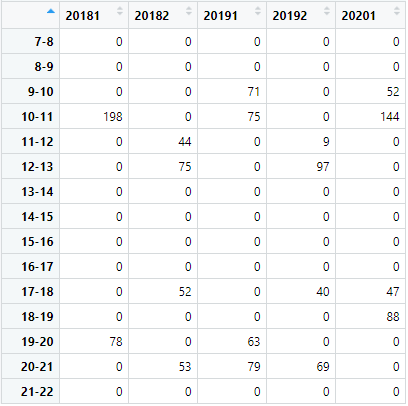
\includegraphics[scale = 0.8]{mat_alumnos_corregidos_EstadisticaIII} %width=\textwidth
%\caption[\textit{Matriz con alumnos de ``Modelos de Supervivencia y Series de Tiempo''}]{\textit{Se puede ver la información del número de alumnos reales de la materia ``Modelos de Supervivencia y Series de Tiempo'' por semestre y por hora.}}\label{matAl_corregidos}
%\end{figure}

%Con el procedimiento descrito pudimos generar vectores por hora. Aplicamos la función \verb@hw()@ en \textit{R} para obtener la demanda de alumnos esperados para el siguiente semestre. En la \figurename{~\ref{vec_alum_sim}} vemos el vector con la demanda de alumnos simulados para el semestre 2020-2 de la materia \textit{Modelos de Supervivencia y Series de Tiempo}.

Con el procedimiento descrito pudimos generar vectores por hora. Aplicamos la función \verb@hw()@ en \textit{R} para obtener la demanda de alumnos esperados para el siguiente semestre. En la \figurename{~\ref{matAl_corregidos_y_sim}} vemos el vector de alumnos simulados (señalado en rojo) para el semestre 2020-2 de la materia \textit{Modelos de Supervivencia y Series de Tiempo}.

Notamos que el valor de la demanda de alumnos es cero cuando en todos los semestres de alguna hora no hay datos. En el ejemplo, es el caso de las 7hrs, 8hrs, 13hrs, 14hrs, 15hrs, 16hrs y 21hrs.

Observando los datos de las 10hrs. vemos que en los semestres pares no hay alumnos, por lo que en la simulación se obtiene únicamente un alumno. Si vemos los datos de las 17hrs vemos que de los 5 semestres en la ventana se tienen alumnos en los semestres pares y en un semestre impar, el número de alumnos simulados para esa hora son 31 alumnos.

Con estos ejemplos podemos ver de manera tangible que el modelo respeta la estacionalidad semestral que tienen los datos.

\begin{figure}[H]
\centering
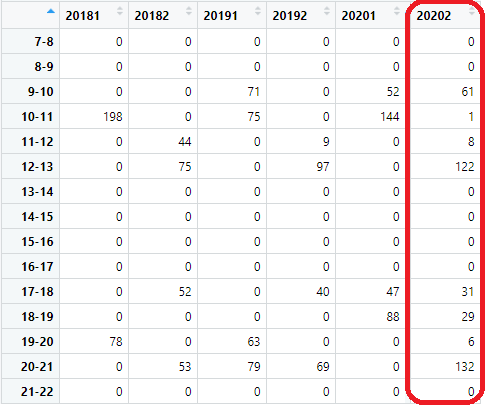
\includegraphics[scale = 0.8]{mat_alumnos_corregidos_con_Sim_EstadisticaIII} %width=\textwidth
\caption[\textit{Matriz con alumnos de ``Modelos de Supervivencia y Series de Tiempo'' y vector con demanda simulada para el 2020-2.}]{\textit{Se puede ver la información del número de alumnos reales de la materia ``Modelos de Supervivencia y Series de Tiempo'' por semestre y por hora. Se señala en rojo el vector con la demanda simulada para el 2020-2.}}\label{matAl_corregidos_y_sim}
\end{figure}

%\begin{figure}[H]
%\centering
%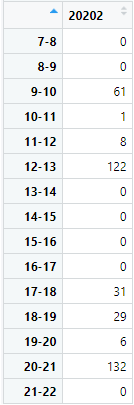
\includegraphics[scale = 0.8]{vec_alum_sim_EstadisticaIII} %width=\textwidth
%\caption[\textit{Vector con demanda simulada para el 2020-2 de ``Modelos de Supervivencia y Series de Tiempo''}]{\textit{Ejemplo de vector con demanda simulada para el 2020-2 de ``Modelos de Supervivencia y Series de Tiempo'': Vemos el vector con el número de alumnos simulados para el 2020-2 de la materia ``Modelos de Supervivencia y Series de Tiempo''}}\label{vec_alum_sim}
%\end{figure}

Obtuvimos vectores con la demanda simulada para cada una de las materias y formamos una matriz de $t \times m$, llamada \textit{mat\_demanda\_alumnos}. Recordemos que $m$ es el número de materias que se van a impartir. En la \figurename{~\ref{matDemandaAlum}} podemos ver un ejemplo de cómo se ve la matriz formada.

Analicemos 2 pares de grupos, primero veamos la columna de \textit{Álgebra Superior II} (2) y la de \textit{Geometría Analítica I} (4). Ambas son materias obligatorias para Actuaría, Matemáticas y Matemáticas Aplicadas. La primera corresponde a semestres pares y la segunda a semestres impares. Notamos que para \textit{Geometría Analítica I}, se tienen alumnos prácticamente en cada hora, pero el número no es muy grande. Para \textit{Álgebra Superior II} hay varias horas con cero alumnos simulados pero hay dos grandes cantidades, una a las 9hrs con 832 alumnos y la otra a las 18hrs con 224 alumnos. Con esta comparación podemos ejemplificar la diferencia entre una materia que corresponde a semestres pares y una de semestres impares.

Ahora analicemos las columnas de \textit{Seminario de Topología A} (3) y \textit{Probabilidad II} (6). La primera es una materia optativa para Matemáticas. La segunda es una materia obligatoria para Actuaría, correspondiente a semestres pares y optativa para Ciencias de la Computación, Matemáticas y Matemáticas Aplicadas. El número total de alumnos simulados para \textit{Seminario de Topología A} es menor a 20, en cambio para \textit{Probabilidad II} se tiene una gran cantidad de alumnos a las 8hrs, 9hrs y 10hrs. Considerando los valores que se tienen en el turno vespertino para \textit{Probabilidad II}, notamos que a las 19hrs también hay una gran cantidad de alumnos. Con esta comparación podemos ejemplificar la diferencia entre una materia obligatoria y una optativa, así como la diferencia entre el turno matutino y vespertino.


\begin{figure}[H]
\centering
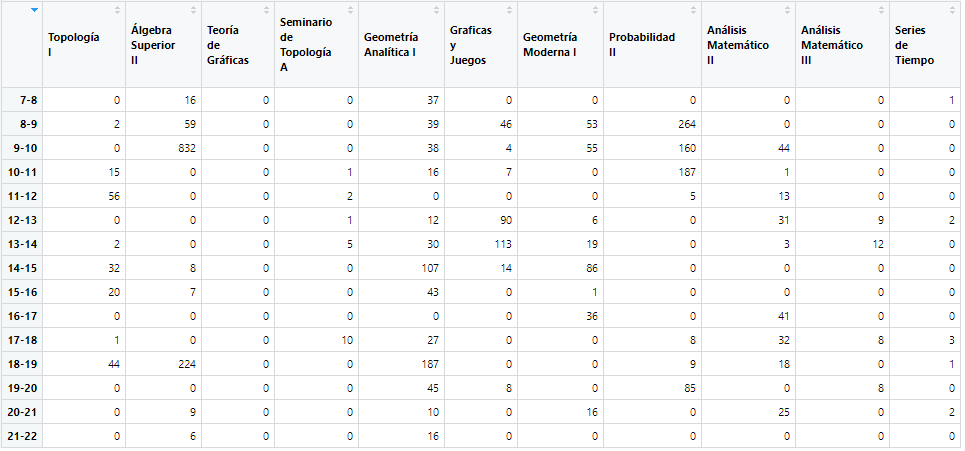
\includegraphics[scale = 0.8]{mat_demanda_alumnos} %width=\textwidth
\caption[\textit{Matriz con demanda simulada para el 2020-2}]{\textit{Se muestra una submatriz de ``mat\_demanda\_alumnos''. Los vectores contienen el número de alumnos simulados para el semestre 2020-2 por hora de algunas materias.}}\label{matDemandaAlum}
\end{figure}


\section{Modelo de Mezcla Gaussiana} \label{sec_GMM}

El modelo de Mezcla Gaussiana también es llamado modelo de mezcla de normales. En él se tienen dos o más distribuciones normales. Se hace una combinación lineal de ellas y se obtiene una nueva distribución de probabilidad.

En \textit{R} se puede generar dicha distribución con la función \verb@normalmixEM()@. La función regresa un objeto de tipo \textit{mixEM} el cual contiene un modelo de una mezcla de distribuciones normales obtenidas por el algoritmo de maximización de la esperanza (EM - \textit{expectation maximization}).

Do Chuong y Batzoglou nos indican, en su artículo \textit{What is the expectation maximization algorithm?} [\ref{ChuongBatzoglou}], que el algoritmo EM es una generalización natural de la estimación por máxima verosimilitud. Ésto para el caso en donde se tiene información incompleta. Recordemos que la máxima verosimilitud se utiliza para encontrar la mejor manera de ajustar una distribución a los datos.

En el algoritmo EM, los parámetros iniciales se toman de los datos reales y se define una distribución \textit{a priori}. Con ellos se obtienen los parámetros de una distribución \textit{a posteriori}. Éstos se convierten en los parámetros iniciales para la siguiente iteración. Este proceso lo realiza la función \verb@normalmixEM()@ hasta encontrar el modelo de mezcla de normales.

Los principales parámetros que recibe la función \verb@normalmixEM()@ son: 
  
  \begin{itemize}
\item[-] \textit{x: } Vector con los datos a los que se les quiere aplicar el modelo.

\item[-] \textit{mu: } Vector con las medias iniciales para el algoritmo EM.

\item[-] \textit{sigma: } Vector con las desviaciones estándar iniciales del modelo.

\item[-] \textit{k: } Número de distribuciones normales que se ajustan a los datos.
\end{itemize}

Cabe mencionar que el objeto de tipo \textit{mixEM} contiene los valores de $\mu$ y $\sigma$ finales. Éstos nos sirven para simular números aleatorios con una distribución normal. Dicha distribución tiene $k$ medias, así como $k$ desviaciones estándar.

En la \figurename{~\ref{GMM_alum_ini}} se puede ver el histograma con el número de alumnos esperados por hora. Los datos corresponden a una matriz \textit{mat\_demanda\_alumnos}. Guardamos el modelo inicial con el comando: \verb@mixmdl_1_D <- normalmixEM(wait_alumnos,k = 4)@.

La línea azul de dicha figura corresponde a la densidad ajustada de 1000 números aleatorios con una distribución normal con 4 medias. El comando para obtener la densidad es: \verb@density(rnorm(1000,mean = mixmdl_1_D$mu,sd = mixmdl_1_D$sigma)@. Se tomaron los valores de $\mu$ y $\sigma$ arrojados por el modelo \textit{mixmdl\_1\_D}. %(ver Sección \ref{SimDemandaAlumnos})
                                                                                                                                                                                                                                                                                                                                                                                                                                                                                


\begin{figure}[h]
\centering
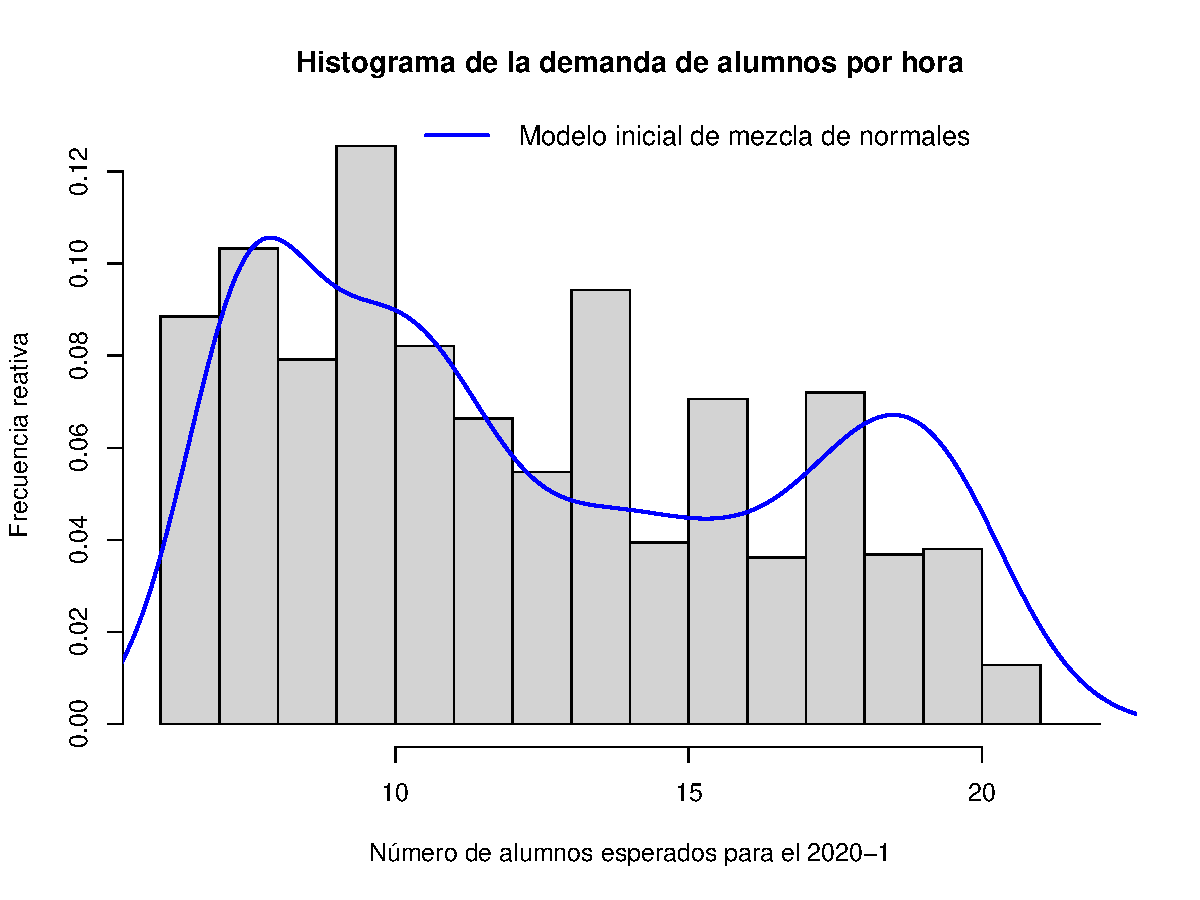
\includegraphics[scale = 0.65]{gmm_alum_ini.pdf} %width=\textwidth
\caption[\textit{Histograma del número de alumnos esperados por hora: Modelo inicial de mezcla de normales}]{\textit{Se muestra el histograma del número de alumnos esperados por hora. La línea azul corresponde a la densidad ajustada de 1000 números aleatorios con la distribución obtenida con el modelo inicial de mezcla de normales.}}\label{GMM_alum_ini}
\end{figure}

En la \figurename{~\ref{GMM_alum_fin}} se puede observar el histograma con el número de alumnos esperados por hora. Los datos corresponden a 5 matrices \textit{mat\_demanda\_alumnos}. Con el comando \verb@mixmdl_D <- normalmixEM(wait_alumnos_final,mixmdl_1_D$mu)@ guardamos el modelo final. En este caso la función recibió los datos del modelo inicial. Los valores de $\mu$ son: $7.49, 10.30, 13.78$ y $17.23$. Para obtener la densidad ajustada, mostrada en la figura (línea azul), utilizamos los valores de $\mu$ y $\sigma$ arrojados por el modelo \textit{mixmdl\_D}.


%Notamos que la densidad se ajusta mejor a los datos. Ésto debido a que para este caso se tiene más información y los valores iniciales son mejores. Se puede ver el pico de las 10hrs, también se observa que se toman en cuenta los picos de las 14hrs, 16hrs y 18hrs.

\begin{figure}[H]
\centering
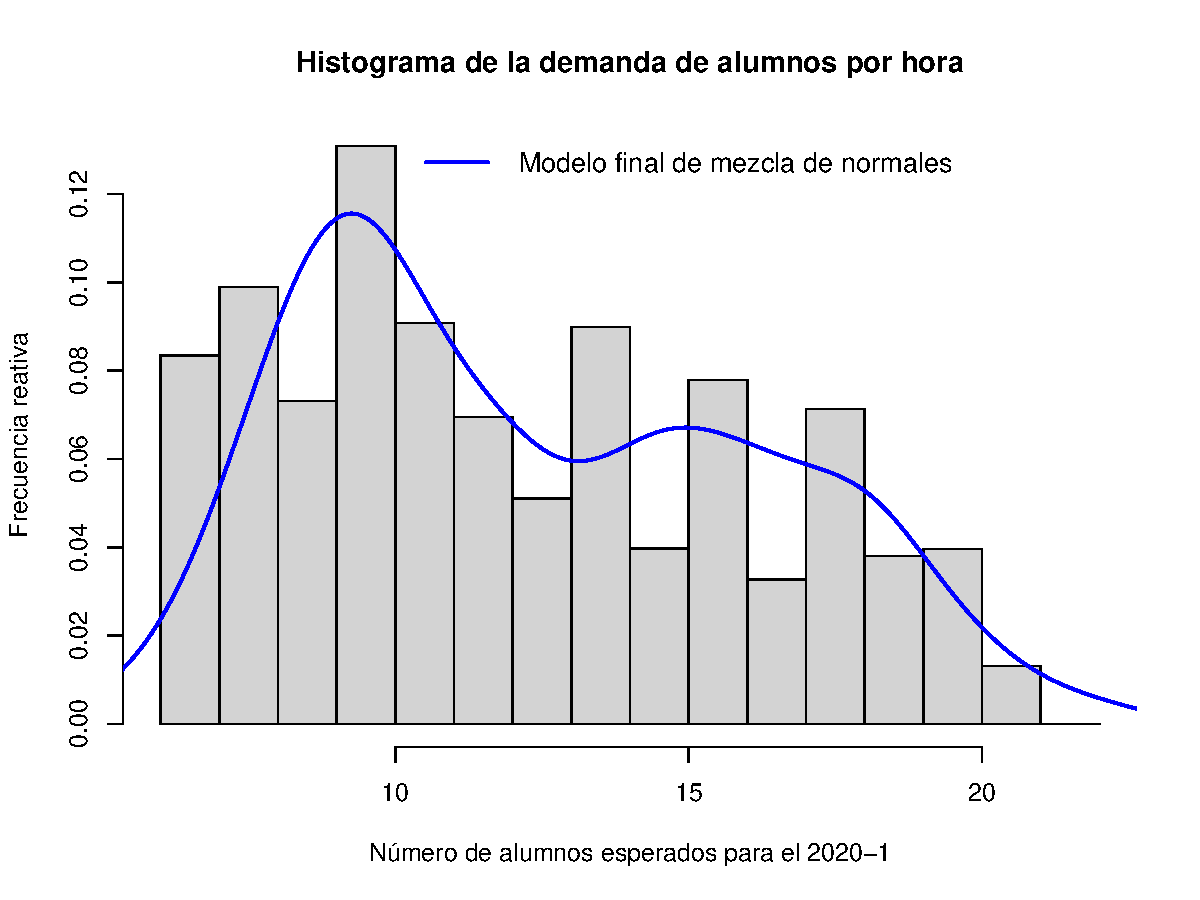
\includegraphics[scale = 0.65]{gmm_alum_fin.pdf} %width=\textwidth
\caption[\textit{Histograma del número de alumnos esperados por hora: Modelo final de mezcla de normales}]{\textit{Se muestra el histograma del número de alumnos esperados por hora. La línea azul corresponde a la densidad ajustada de 1000 números aleatorios con la distribución obtenida con el modelo final de mezcla de normales.}}\label{GMM_alum_fin}
\end{figure}

Notamos que la densidad se ajusta mejor a los datos. Ésto debido a que para este caso se tiene más información y los valores iniciales son mejores. Se puede ver el pico de las 10hrs, también se observa que se toman en cuenta los picos de las 14hrs, 16hrs y 18hrs.

%En la \figurename{~\ref{GMM_ini_fin}} se pueden ver dos histogramas con el número de alumnos esperados por hora.
                                                                                                                                                                                                                                                                                                                                                                                                                                                                                %\begin{figure}[H]
                                                                                                                                                                                                                                                                                                                                                                                                                                                                                %\centering
                                                                                                                                                                                                                                                                                                                                                                                                                                                                                %\subfigure[\textit{Modelo inicial}]{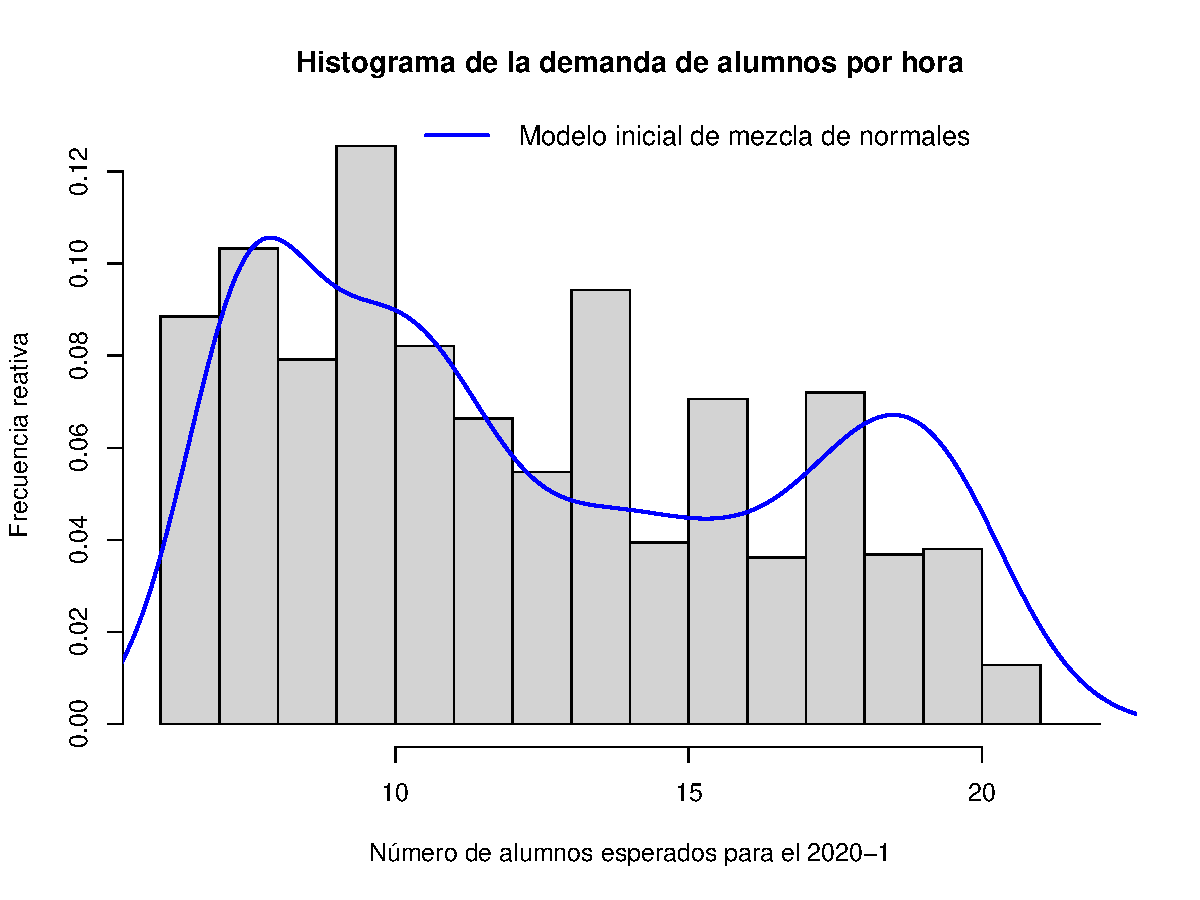
\includegraphics[width=12cm]{gmm_alum_ini.pdf}} %%Ping\"uino %%[angle=30]
                                                                                                                                                                                                                                                                                                                                                                                                                                                                                %	\subfigure[\textit{Modelo final}]{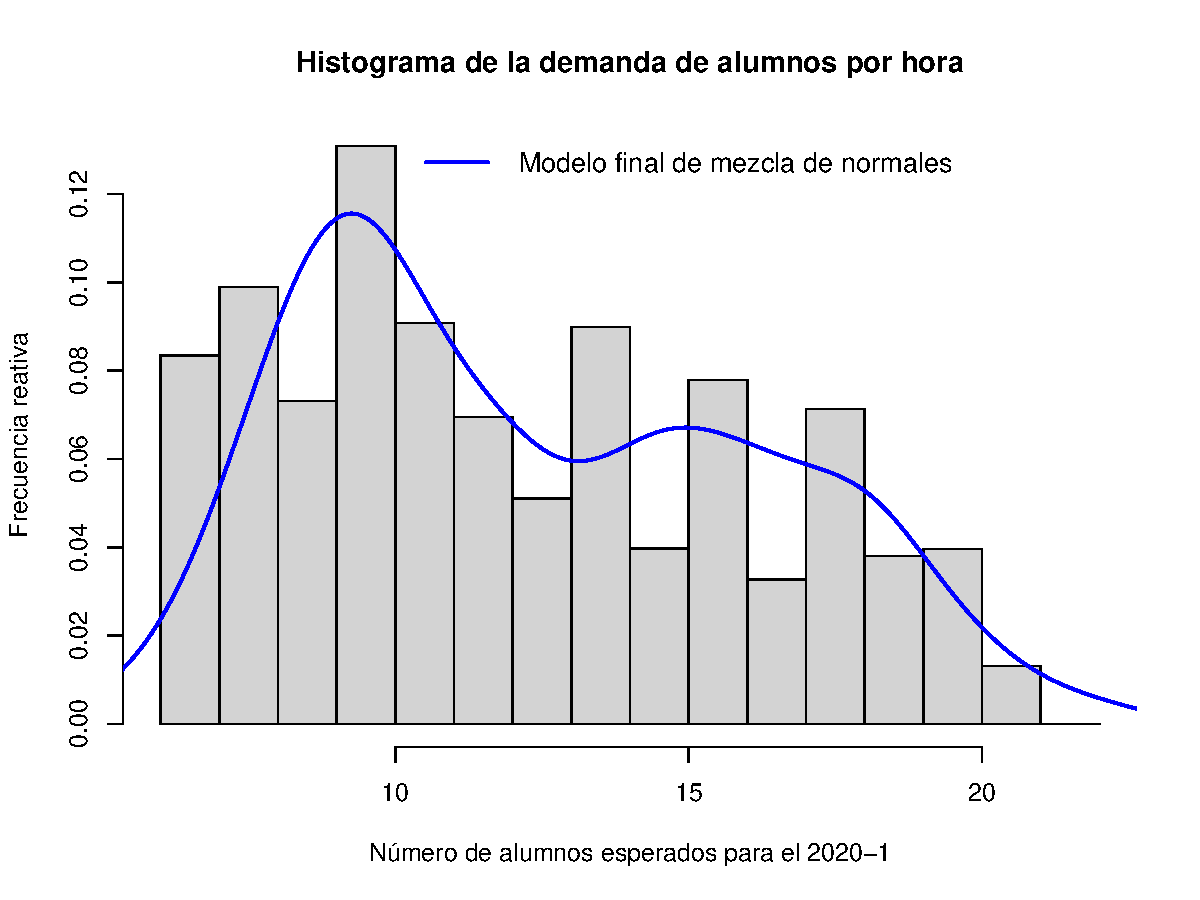
\includegraphics[width=12cm]{gmm_alum_fin.pdf}}
                                                                                                                                                                                                                                                                                                                                                                                                                                                                                %	\caption[\textit{Histogramas con el número de alumnos esperados por hora}]{\textit{Se muestran dos histogramas con el número de alumnos esperados por hora. Cada uno tiene la densidad ajustada de 1000 números aleatorios con la distribución obtenida con el modelo de mezcla de normales.}}\label{GMM_ini_fin}
                                                                                                                                                                                                                                                                                                                                                                                                                                                                                %\end{figure}
                                                                                                                                                                                                                                                                                                                                                                                                                                                                                
                                                                                                                                                                                                                                                                                                                                                                                                                                                                                
                                                                                                                                                                                                                                                                                                                                                                                                                                                                                %En la \figurename{~\ref{GMM_inicial_final}} se muestran dos histogramas con los datos iniciales y finales, respectivamente. Las líneas verdes corresponden al ajuste con la función \verb@density()@ en \textit{R} y las azules al modelo de mezcla de normales.
                                                                                                                                                                                                                                                                                                                                                                                                                                                                                %
                                                                                                                                                                                                                                                                                                                                                                                                                                                                                %\begin{figure}[H]
                                                                                                                                                                                                                                                                                                                                                                                                                                                                                %\centering
                                                                                                                                                                                                                                                                                                                                                                                                                                                                                %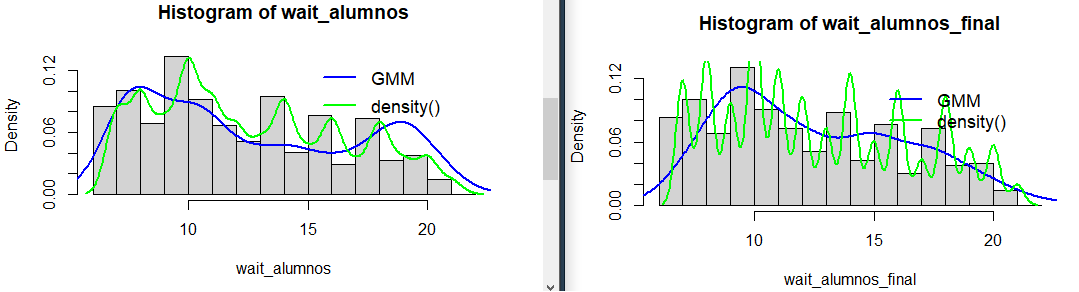
\includegraphics[width=\textwidth]{histograma_y_GMM} %scale = 1
                                                                                                                                                                                                                                                                                                                                                                                                                                                                                %\caption{\textit{Mezcla de normales inicial y final}}\label{GMM_inicial_final}
                                                                                                                                                                                                                                                                                                                                                                                                                                                                                %\end{figure}
                                                                                                                                                                                                                                                                                                                                                                                                                                                                                
                                                                                                                                                                                                                                                                                                                                                                                                                                                                                %\url{https://www.youtube.com/watch?v=REypj2sy_5U&ab_channel=VictorLavrenko}
                                                                                                                                                                                                                                                                                                                                                                                                                                                                                %
                                                                                                                                                                                                                                                                                                                                                                                                                                                                                %\url{https://www.youtube.com/watch?v=iQoXFmbXRJA&ab_channel=VictorLavrenko}
                                                                                                                                                                                                                                                                                                                                                                                                                                                                                %
                                                                                                                                                                                                                                                                                                                                                                                                                                                                                %\url{https://www.youtube.com/watch?v=pYxNSUDSFH4&ab_channel=StatQuestwithJoshStarmer}
                                                                                                                                                                                                                                                                                                                                                                                                                                                                                %
                                                                                                                                                                                                                                                                                                                                                                                                                                                                                %\url{https://www.youtube.com/watch?v=XepXtl9YKwc&ab_channel=StatQuestwithJoshStarmer} %%  The goal of the maximum likelihood is to find the optimal way to fit a distribution to the data.
                                                                                                                                                                                                                                                                                                                                                                                                                                                                                %
                                                                                                                                                                                                                                                                                                                                                                                                                                                                                %\url{https://www.youtube.com/watch?v=s3sTSA_GXV8&ab_channel=InstitutodeInformaticaUACh}
                                                                                                                                                                                                                                                                                                                                                                                                                                                                                %
                                                                                                                                                                                                                                                                                                                                                                                                                                                                                %\url{https://www.youtube.com/watch?v=_igVkRP9TFE&ab_channel=InstitutodeInformaticaUACh}
                                                                                                                                                                                                                                                                                                                                                                                                                                                                                %
                                                                                                                                                                                                                                                                                                                                                                                                                                                                                %\url{https://natureofcode.com/book/chapter-9-the-evolution-of-code/}
                                                                                                                                                                                                                                                                                                                                                                                                                                                                                
                                                                                                                                                                                                                                                                                                                                                                                                                                                                                
                                                                                                                                                                                                                                                                                                                                                                                                                                                                                
                                                                                                                                                                                                                                                                                                                                                                                                                                                                                %\begin{figure}[H]
                                                                                                                                                                                                                                                                                                                                                                                                                                                                                %\centering
                                                                                                                                                                                                                                                                                                                                                                                                                                                                                %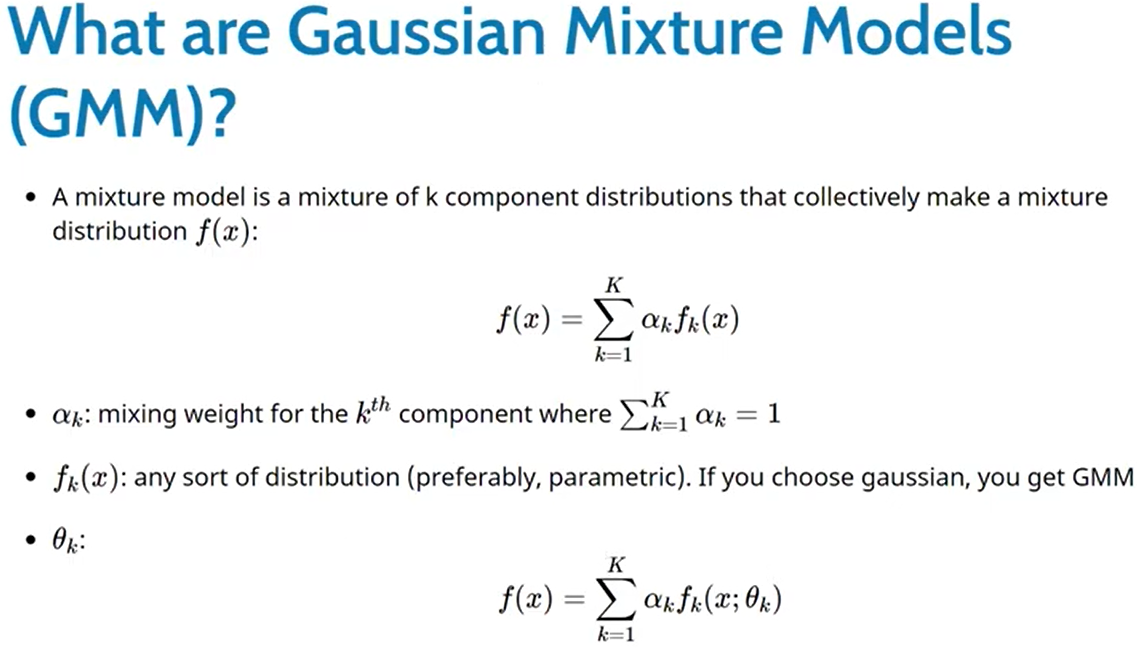
\includegraphics[scale = 0.5]{GMM_1} %width=\textwidth
                                                                                                                                                                                                                                                                                                                                                                                                                                                                                %\caption{\textit{GMM 1}}
                                                                                                                                                                                                                                                                                                                                                                                                                                                                                %\end{figure}
                                                                                                                                                                                                                                                                                                                                                                                                                                                                                %
                                                                                                                                                                                                                                                                                                                                                                                                                                                                                %\begin{figure}[H]
                                                                                                                                                                                                                                                                                                                                                                                                                                                                                %\centering
                                                                                                                                                                                                                                                                                                                                                                                                                                                                                %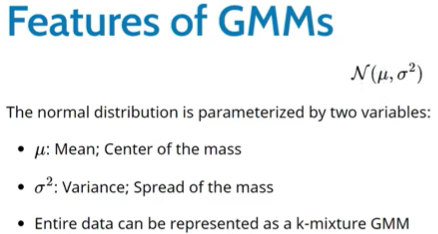
\includegraphics[scale = 0.5]{GMM_2} %width=\textwidth
                                                                                                                                                                                                                                                                                                                                                                                                                                                                                %\caption{\textit{GMM 2}}
                                                                                                                                                                                                                                                                                                                                                                                                                                                                                %\end{figure}
                                                                                                                                                                                                                                                                                                                                                                                                                                                                                %
                                                                                                                                                                                                                                                                                                                                                                                                                                                                                %\begin{figure}[H]
                                                                                                                                                                                                                                                                                                                                                                                                                                                                                %\centering
                                                                                                                                                                                                                                                                                                                                                                                                                                                                                %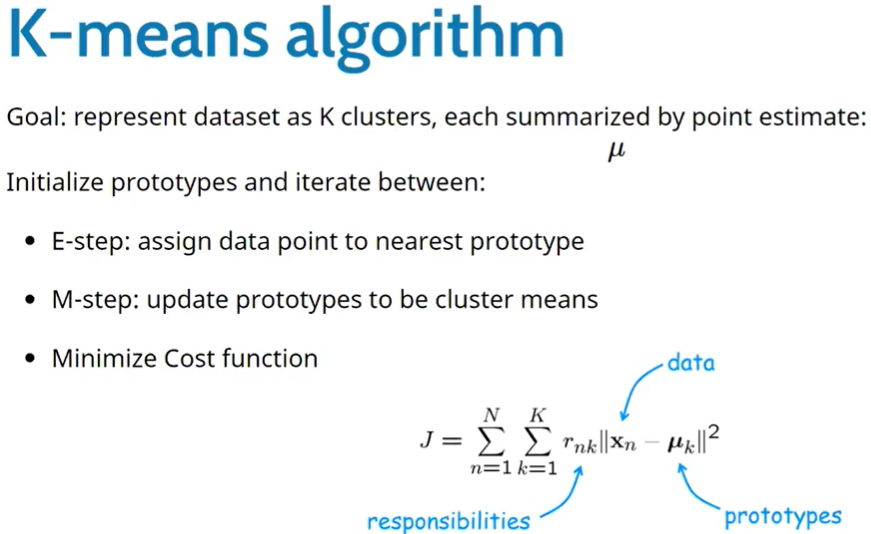
\includegraphics[scale = 0.5]{GMM_3} %width=\textwidth
                                                                                                                                                                                                                                                                                                                                                                                                                                                                                %\caption{\textit{GMM 3}}
                                                                                                                                                                                                                                                                                                                                                                                                                                                                                %\end{figure}
                                                                                                                                                                                                                                                                                                                                                                                                                                                                                %
                                                                                                                                                                                                                                                                                                                                                                                                                                                                                %\begin{figure}[H]
                                                                                                                                                                                                                                                                                                                                                                                                                                                                                %\centering
                                                                                                                                                                                                                                                                                                                                                                                                                                                                                %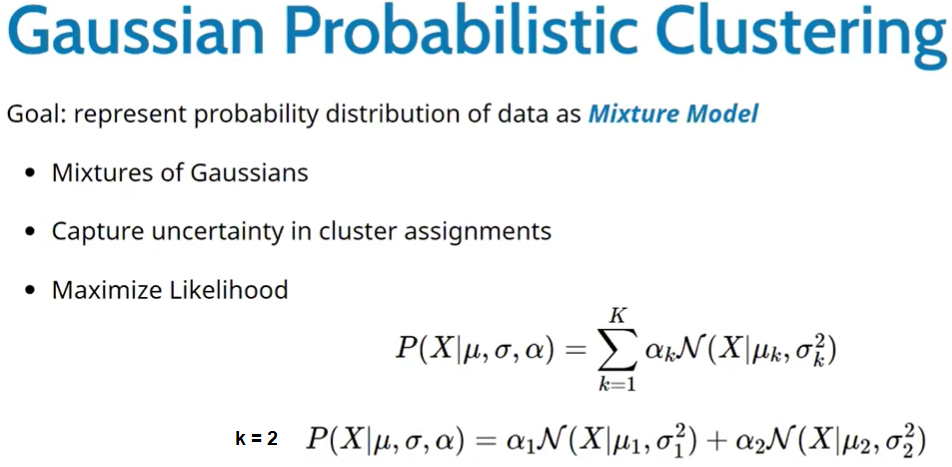
\includegraphics[scale = 0.5]{GMM_4} %width=\textwidth
                                                                                                                                                                                                                                                                                                                                                                                                                                                                                %\caption{\textit{GMM 4}}
                                                                                                                                                                                                                                                                                                                                                                                                                                                                                %\end{figure}
                                                                                                                                                                                                                                                                                                                                                                                                                                                                                %
                                                                                                                                                                                                                                                                                                                                                                                                                                                                                %\begin{figure}[H]
                                                                                                                                                                                                                                                                                                                                                                                                                                                                                %\centering
                                                                                                                                                                                                                                                                                                                                                                                                                                                                                %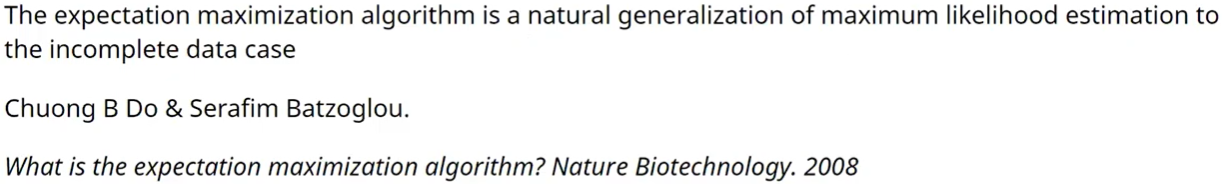
\includegraphics[scale = 0.5]{GMM_5} %width=\textwidth
                                                                                                                                                                                                                                                                                                                                                                                                                                                                                %\caption{\textit{GMM 5}}
                                                                                                                                                                                                                                                                                                                                                                                                                                                                                %\end{figure}
                                                                                                                                                                                                                                                                                                                                                                                                                                                                                %
                                                                                                                                                                                                                                                                                                                                                                                                                                                                                %\begin{figure}[H]
                                                                                                                                                                                                                                                                                                                                                                                                                                                                                %\centering
                                                                                                                                                                                                                                                                                                                                                                                                                                                                                %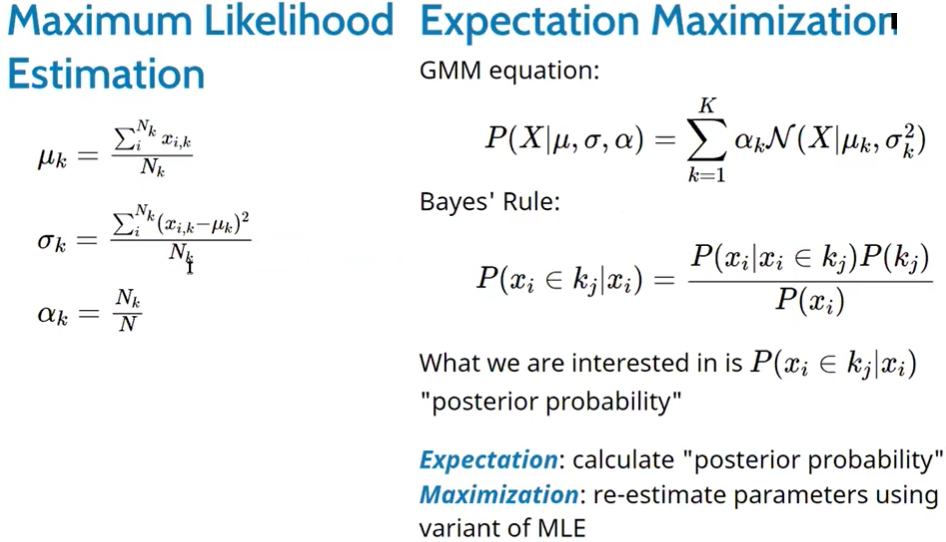
\includegraphics[scale = 0.5]{GMM_6} %width=\textwidth
                                                                                                                                                                                                                                                                                                                                                                                                                                                                                %\caption{\textit{GMM 6}}
                                                                                                                                                                                                                                                                                                                                                                                                                                                                                %\end{figure}
                                                                                                                                                                                                                                                                                                                                                                                                                                                                                %
                                                                                                                                                                                                                                                                                                                                                                                                                                                                                %\begin{figure}[H]
                                                                                                                                                                                                                                                                                                                                                                                                                                                                                %\centering
                                                                                                                                                                                                                                                                                                                                                                                                                                                                                %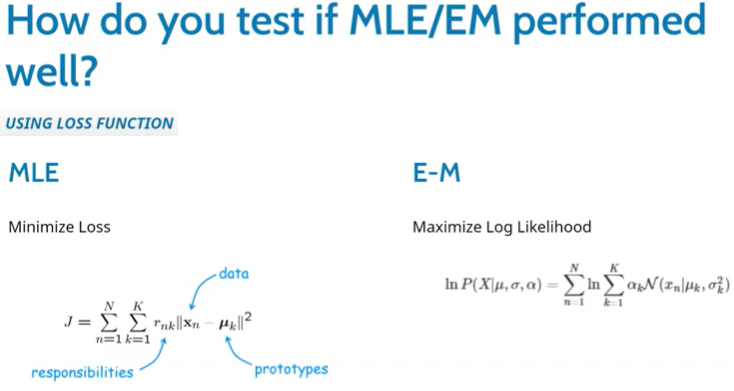
\includegraphics[scale = 0.5]{GMM_7} %width=\textwidth
                                                                                                                                                                                                                                                                                                                                                                                                                                                                                %\caption{\textit{GMM 7}}
                                                                                                                                                                                                                                                                                                                                                                                                                                                                                %\end{figure}
                                                                                                                                                                                                                                                                                                                                                                                                                                                                                
                                                                                                                                                                                                                                                                                                                                                                                                                                                                                El modelo de mezcla de normales lo utilizamos para simular los esqueletos de los horarios. En las siguientes secciones veremos cómo aplicamos la función \verb@normalmixEM()@ para obtener la matriz \textit{mat\_esqueleto}.
                                                                                                                                                                                                                                                                                                                                                                                                                                                                                
                                                                                                                                                                                                                                                                                                                                                                                                                                                                                
                                                                                                                                                                                                                                                                                                                                                                                                                                                                                \section{Obtención de $D'$ y $D_{0}$} \label{GMM_D}

Los esqueletos que vamos a simular dependen de la demanda de alumnos. En esta sección vamos a mostrar 4 diferentes metodologías que probamos para poder simular adecuadamente los esqueletos. Ésto basándonos en el número de alumnos simulados para el siguiente semestre. %Al final de esta sección, vamos a describir el método con el que generamos la matriz \textit{mat\_esqueleto}.


Definimos las siguientes matrices:

\begin{itemize}
\item[-] $D': $ Matriz de $t \times m$, con la demanda simulada por alguna de las 4 metodologías.
                                                                                                                                                                                                                                                                                                                                                                                                                                                                                  
                                                                                                                                                                                                                                                                                                                                                                                                                                                                                  \item[-] $D^{0}: $ Matriz de $t \times m$, con la cual se va a comparar $D'$ para calificarla. Esta matriz se obtiene haciendo el promedio entre una matriz \textit{mat\_demanda\_alumnos} y una matriz de demanda de alumnos, obtenida con el modelo de mezcla de normales. %(ver Sección \ref{SimDemandaAlumnos}) (ver Sección \ref{sec_GMM})
\end{itemize}

La calificación de las metodologías depende de la diferencia relativa entre $D^{0}$ y $D'$. Los pasos que seguimos para obtener las calificiones son:
                                                                                                                                                                                                                                                                                                                                                                                                                                                                                    
                                                                                                                                                                                                                                                                                                                                                                                                                                                                                    \begin{enumerate}
                                                                                                                                                                                                                                                                                                                                                                                                                                                                                  \item Definir la matriz $C$, de $t \times m$. Esta matriz va a guardar las calificaciones por grupo de $D'$.

\item Para cada $C_{h,j}$ guardar el valor de $\dfrac{D_{h,j}^{0} - D'_{h,j}}{D_{h,j}^{0}}$. 
                                                                                                                                                                                                                                                                                                                                                                                                                                                                                
                                                                                                                                                                                                                                                                                                                                                                                                                                                                                \item Si $D_{h,j}^{0} = 0$ entonces $C_{h,j} = 1$ si faltan alumnos y $C_{h,j} = -1$ si sobran alumnos, es decir: $C_{h,j} = \left \{ \begin{matrix} 1 & \mbox{si }D_{h,j}^{0} > D'_{h,j}\\ 
-1 & \mbox{si }D_{h,j}^{0} < D'_{h,j}\\ 0 & \mbox{e.o.c. }\end{matrix}\right.$
                                                                                                                                                                                                                                                                                                                                                                                                                                                                                    
                                                                                                                                                                                                                                                                                                                                                                                                                                                                                    
                                                                                                                                                                                                                                                                                                                                                                                                                                                                                    
                                                                                                                                                                                                                                                                                                                                                                                                                                                                                    \item Definir el vector \textit{vec\_calif\_x\_materia} con el promedio por columna de $C$. Este vector guarda las calificaciones por materia de $D'$.
\end{enumerate}

Para cada metodología, realizamos 10 simulaciones y calificamos las matrices $D'$ generadas. Con este procedimiento obtuvimos 4 matrices de 10 renglones y $m$ columnas. Graficamos cada matriz con la función \verb@matplot()@ en \textit{R}. Cada gráfica contiene $m$ líneas con 10 puntos cada una. A continuación mostramos las 4 gráficas.
                                                                                                                                                                                                                                                                                                                                                                                                                                                                                  
                                                                                                                                                                                                                                                                                                                                                                                                                                                                                  En la \figurename{~\ref{fig_metodo_A}} vemos las calificaciones por materia de la metodología A. Notamos que se encuentran entre -5 y 1. Ésto quiere decir que en promedio con este método sobra hasta un 500\% de alumnos y falta casi un 100\% al hacer la simulación.


\begin{figure}[h]
\centering
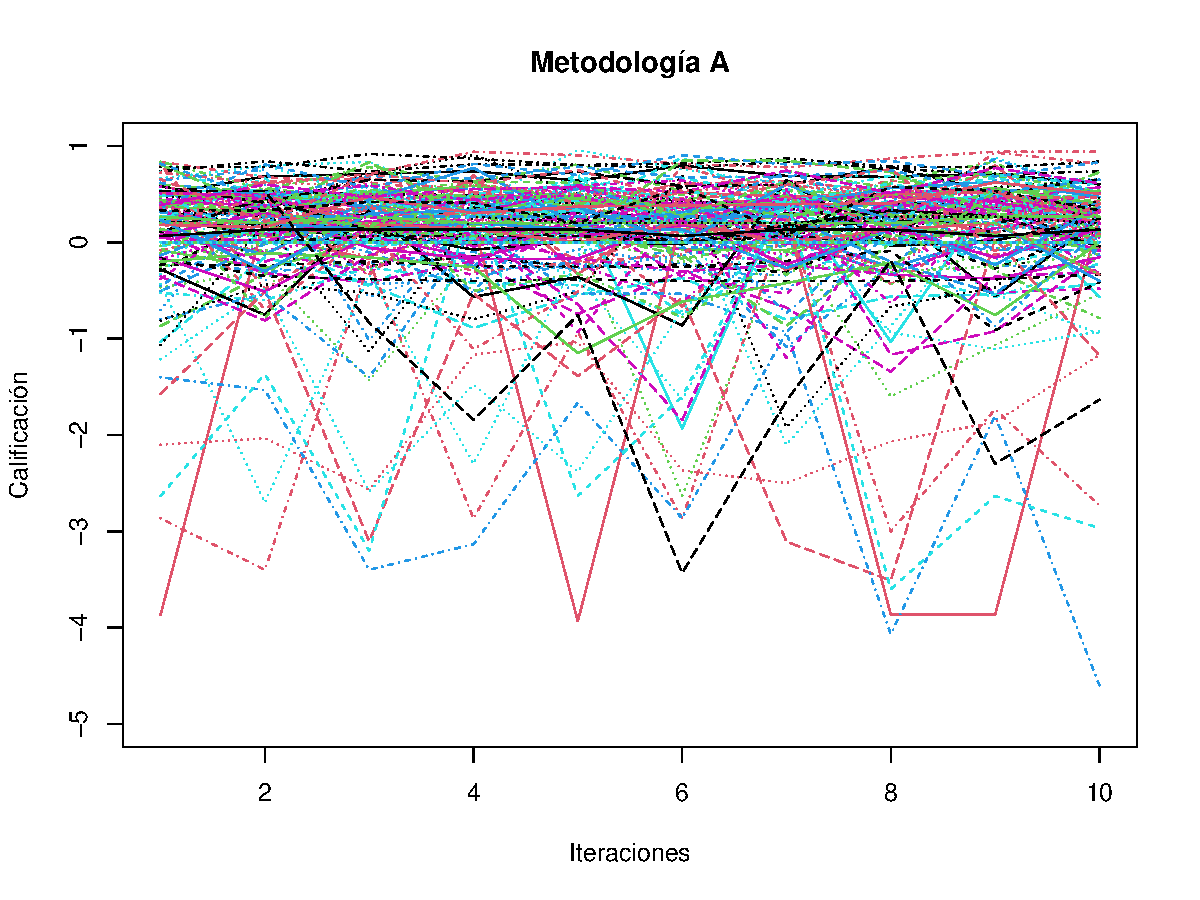
\includegraphics[scale = 0.65]{matplot_metodo_A.pdf} %width=\textwidth
\caption[\textit{Calificaciones metodología A}]{\textit{Se muestran las calificaciones por materia de la metodología A. Las calificaciones se encuentran entre -5 y 1.}}\label{fig_metodo_A}
\end{figure}


En la \figurename{~\ref{fig_metodo_B}} vemos las calificaciones por materia de la metodología B. Notamos que se encuentran entre -0.5 y 0.8. Ésto quiere decir que en promedio con este método sobra hasta un 50\% de alumnos y falta casi un 80\% al hacer la simulación.

\begin{figure}[H]
\centering
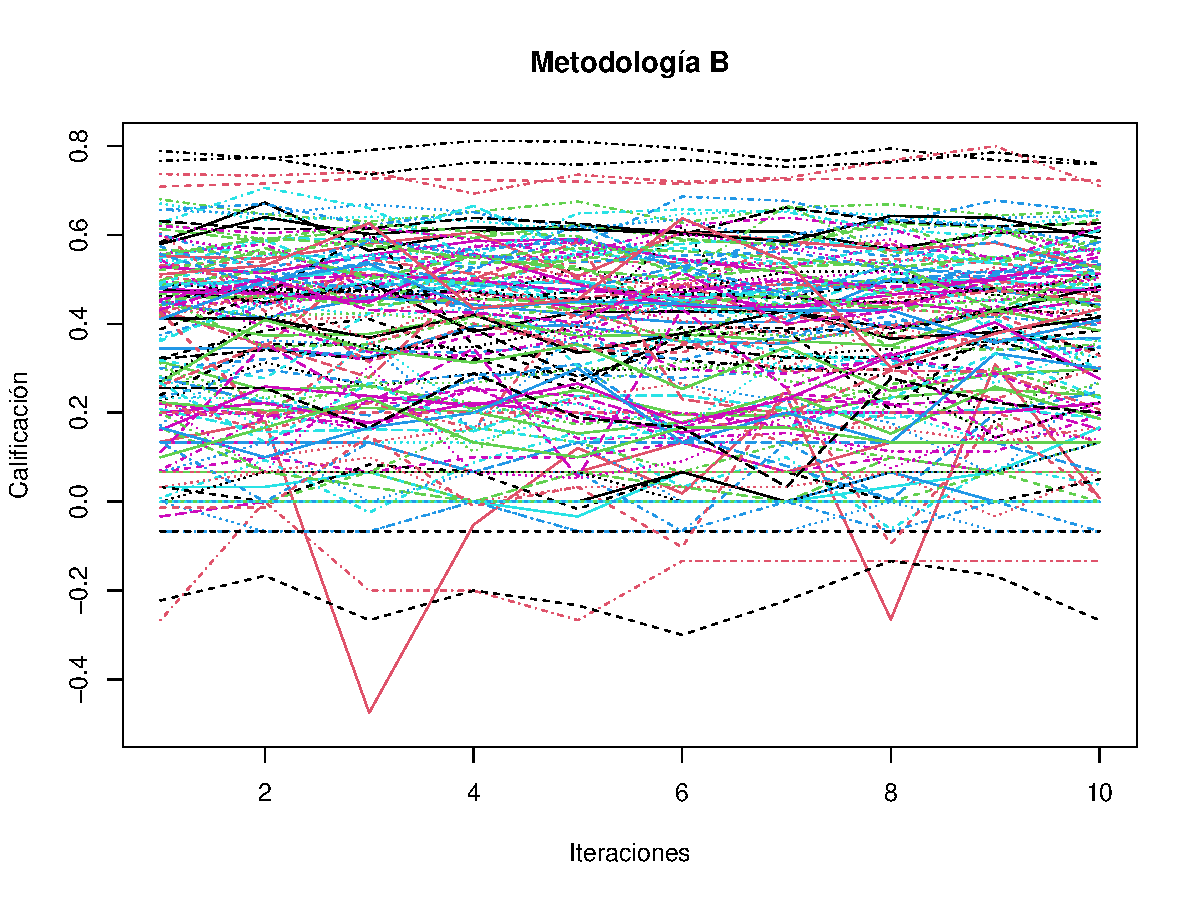
\includegraphics[scale = 0.65]{matplot_metodo_B.pdf} %width=\textwidth
\caption[\textit{Calificaciones metodología B}]{\textit{Se muestran las calificaciones por materia de la metodología B. Las calificaciones se encuentran entre -0.5 y 0.8. Hay una mayor concentración entre 0.4 y 0.6.}}\label{fig_metodo_B}
\end{figure}

En la \figurename{~\ref{fig_metodo_C}} vemos las calificaciones por materia de la metodología C. Notamos que, al igual que en la metodología B, las calificaciones se encuentran entre -0.5 y 0.8. En este caso observamos que hay una mayor concentración de materias (líneas) entre 0.5 y 0.8. Ésto comparado con el método B que tiene una mayor concentración entre 0.4 y 0.6.

\begin{figure}[H]
\centering
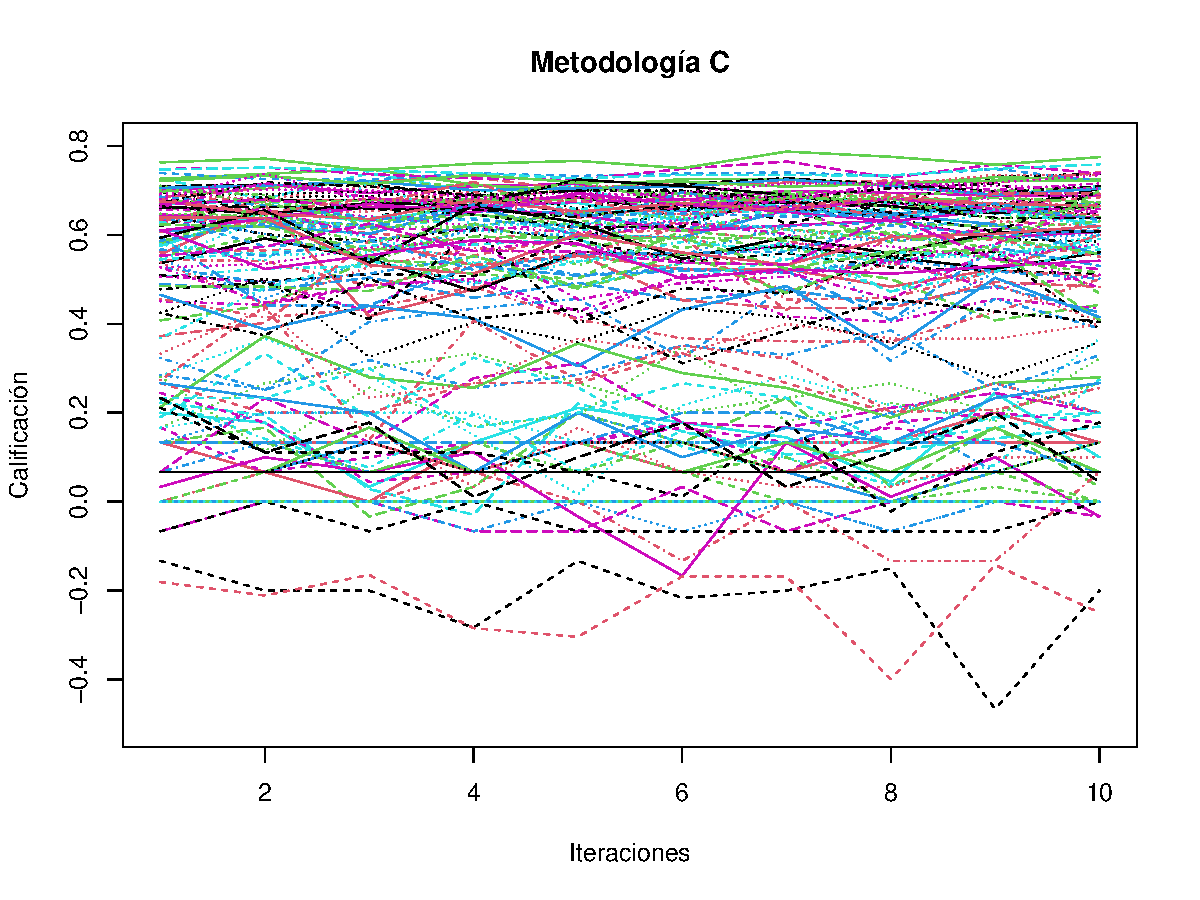
\includegraphics[scale = 0.65]{matplot_metodo_C.pdf} %width=\textwidth
\caption[\textit{Calificaciones metodología C}]{\textit{Se muestran las calificaciones por materia de la metodología C.}}\label{fig_metodo_C}
\end{figure}

En la \figurename{~\ref{fig_metodo_D}} vemos las calificaciones por materia de la metodología D. Notamos que se encuentran entre -6 y 0.4. Ésto quiere decir que en promedio con este método sobra hasta un 600\% de alumnos y falta casi un 40\% al hacer la simulación. Podemos observar que sólo una materia tiene calificaciones por debajo de -3. En general todas se concentran entre -2.5 y 0.4.


\begin{figure}[h]
\centering
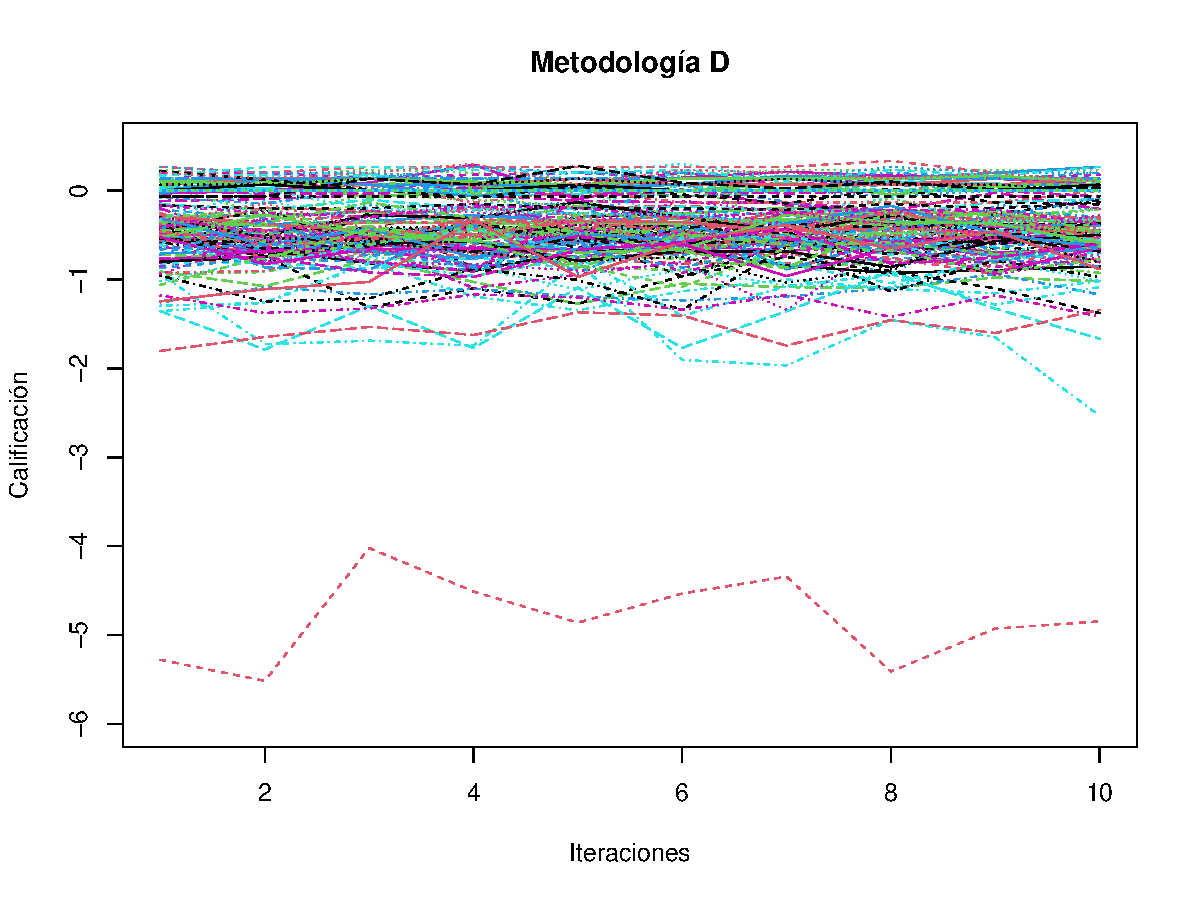
\includegraphics[scale = 0.65]{matplot_metodo_D.pdf} %width=\textwidth
\caption[\textit{Calificaciones metodología D}]{\textit{Se muestran las calificaciones por materia de la metodología D.}}\label{fig_metodo_D}
\end{figure}


Decidimos analizar las metodologías $B$ y $C$ ya que son las que muestran las mejores calificaciones. Para ello graficamos las matrices de calificaciones con la función \verb@heatmap()@ en \textit{R}. Cabe aclarar que las matrices de calificaciones están ordenadas de menor a mayor por renglones. En la \figurename{~\ref{fig_heatmap_B}} vemos el correspondiente a la metodología $B$. En la \figurename{~\ref{fig_heatmap_C}} vemos el \textit{heatmap} referente a la metodología $C$.


%\begin{figure}[H]
%\centering
%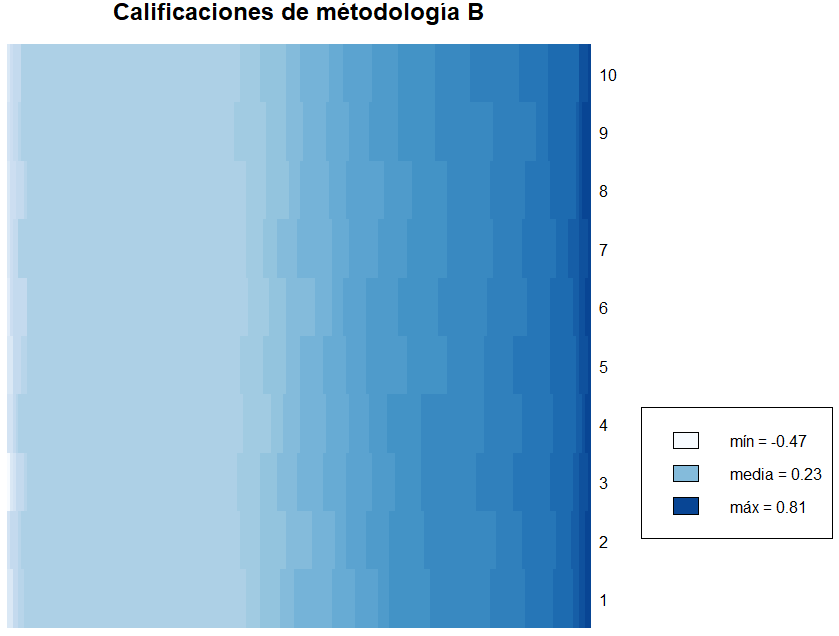
\includegraphics[scale = 0.55]{heatmap_metodo_B_2} %width=\textwidth
%\caption[\textit{Heatmap metodología B}]{\textit{Se muestra el heatmap de las calificaciones por materia de la metodología B.}}\label{fig_heatmap_B}
%\end{figure}
%
%\begin{figure}[H]
%\centering
%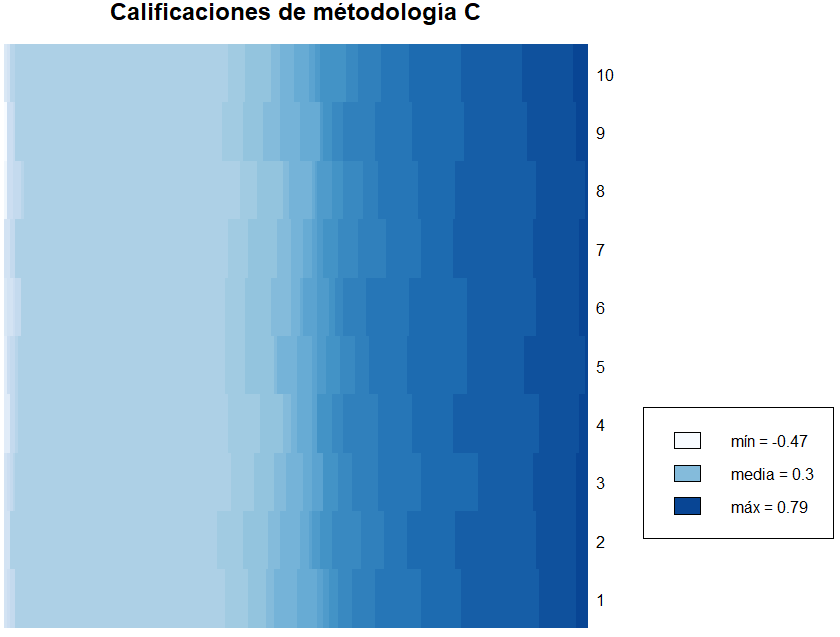
\includegraphics[scale = 0.55]{heatmap_metodo_C_2} %width=\textwidth
%\caption[\textit{Heatmap metodología C}]{\textit{Se muestra el heatmap de las calificaciones por materia de la metodología C.}}\label{fig_heatmap_C}
%\end{figure}


Para elegir entre las dos metodologías, tomamos en cuenta que el error relativo estuviera más cercano a cero. Al ver ambos \textit{heatmaps} observamos que el correspondiente al método $B$ es más claro que el del método $C$. Por lo que elegimos la metodología $B$ para simular los esqueletos. %En la siguiente sección explicaremos el procedimiento que seguimos para ésta metodología.
                                                                                                                                                                                                                                                                                                                                                                                                                                                                                  
                                                                                                                                                                                                                                                                                                                                                                                                                                                                                  En la metodología $B$ la matriz $D'$ es una matriz \textit{mat\_demanda\_alumnos}. La matriz \textit{mat\_esqueleto} se genera con el modelo de mezcla de normales. En las siguientes secciones se describe a detalle el procedimiento que seguimos para obtener la matriz \textit{mat\_esqueleto}. %Es por ello que se genera con el procedimiento descrito en la Sección \ref{SimDemandaAlumnos}. visto en la Sección \ref{sec_GMM}

\begin{figure}[H]
\centering
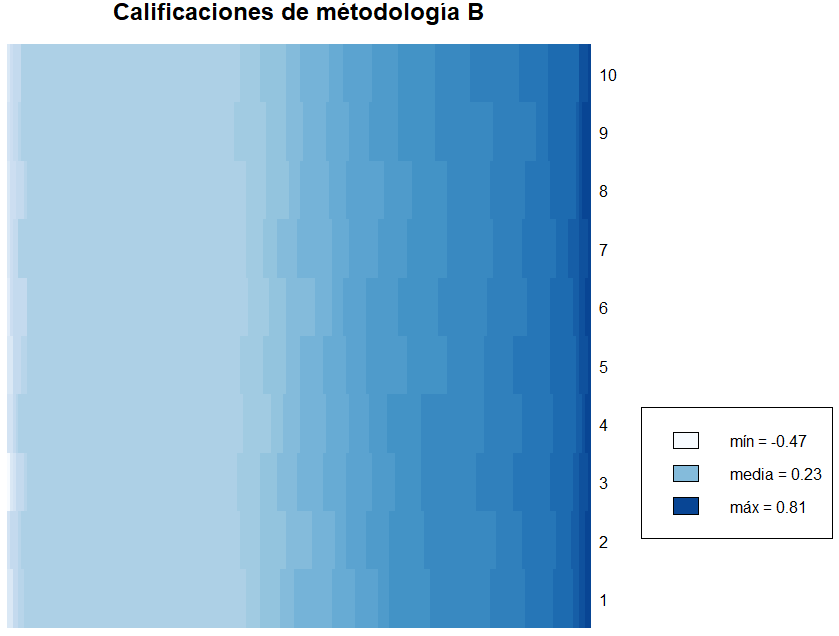
\includegraphics[scale = 0.65]{heatmap_metodo_B_2} %width=\textwidth
\caption[\textit{Heatmap metodología B}]{\textit{Se muestra el heatmap de las calificaciones por materia de la metodología B.}}\label{fig_heatmap_B}
\end{figure}

\begin{figure}[H]
\centering
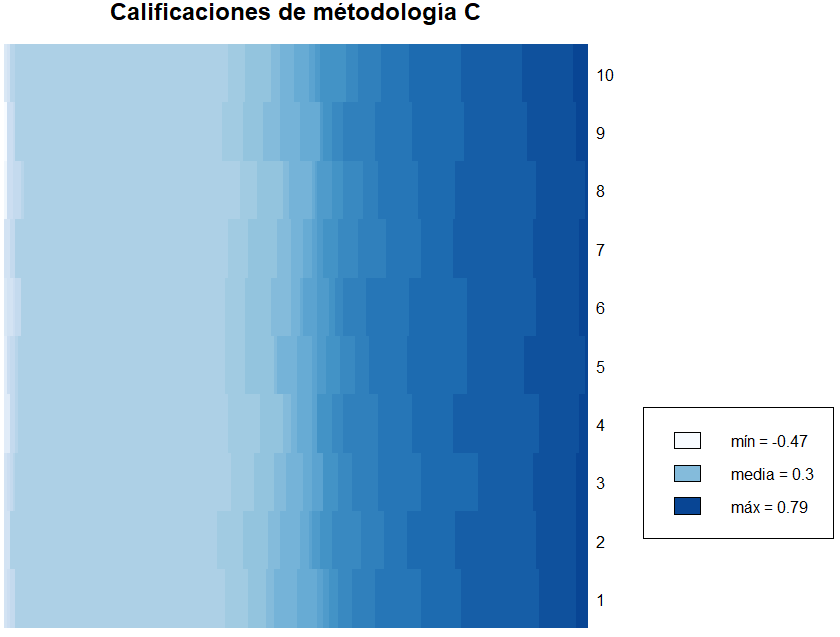
\includegraphics[scale = 0.65]{heatmap_metodo_C_2} %width=\textwidth
\caption[\textit{Heatmap metodología C}]{\textit{Se muestra el heatmap de las calificaciones por materia de la metodología C.}}\label{fig_heatmap_C}
\end{figure}